%
% This is the Appendix A file (appA.tex)
%
\appendix{Brazil Plots} \label{apdx:A}

    In \Cref{sec:app2} we showed Brazil-plots from dataset \texttt{wnd} (\Cref{fig:brazil_prob_wnd})
    and \texttt{mms} (\Cref{fig:brazil_prob_mms}). Here we show the Brazil-plot from rest of the
    datasets mentioned in \Cref{chap:chap4}.
    
    We observe that for 2.5-D simulations because of low values of $R_{\rm p}$ and $\beta_{\parallel
    \rm p}$, the instability thresholds are not very well aligned with the distribution of the
    plasma. However, the plasma in all cases are well confined. For the 3-D case where the
    propagation vector is not restrained, we do observe a Brazil plot which is very similar to that
    observed in space plasma data.
    \begin{figure}
        \begin{center}
            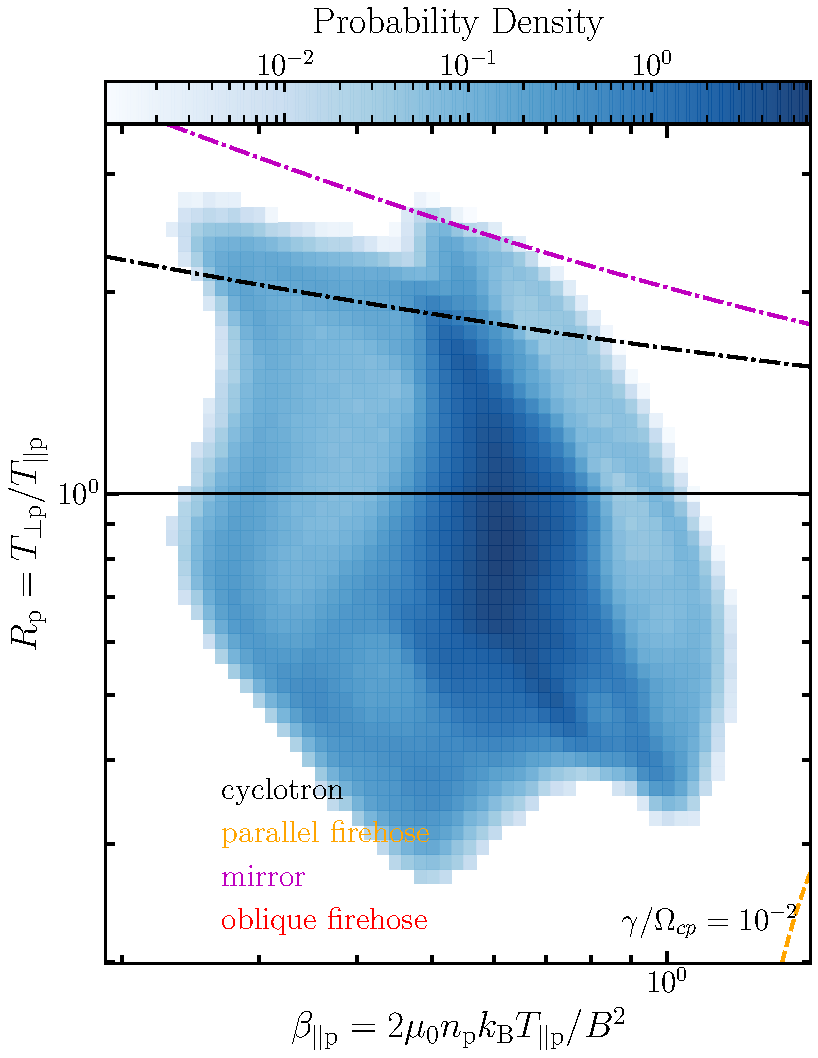
\includegraphics[width=1\textwidth]{figures/apdxA/brazil_prob_2dip.pdf}
            \caption[Brazil-plot of \texttt{149p6} dataset]{Plot of estimated probability density,
            $\Tilde{p}$ of ($R_{\rm p}, \beta_{\parallel \rm p}$) for \texttt{149p6} dataset and
            thresholds associated with different instabilities for threshold value of
            $\gamma_{\max}/\Omega_{\rm cp} = 10^{-3}$.}
            \label{fig:brazil_prob_2dip}
        \end{center}
    \end{figure}

    \begin{figure}
        \begin{center}
            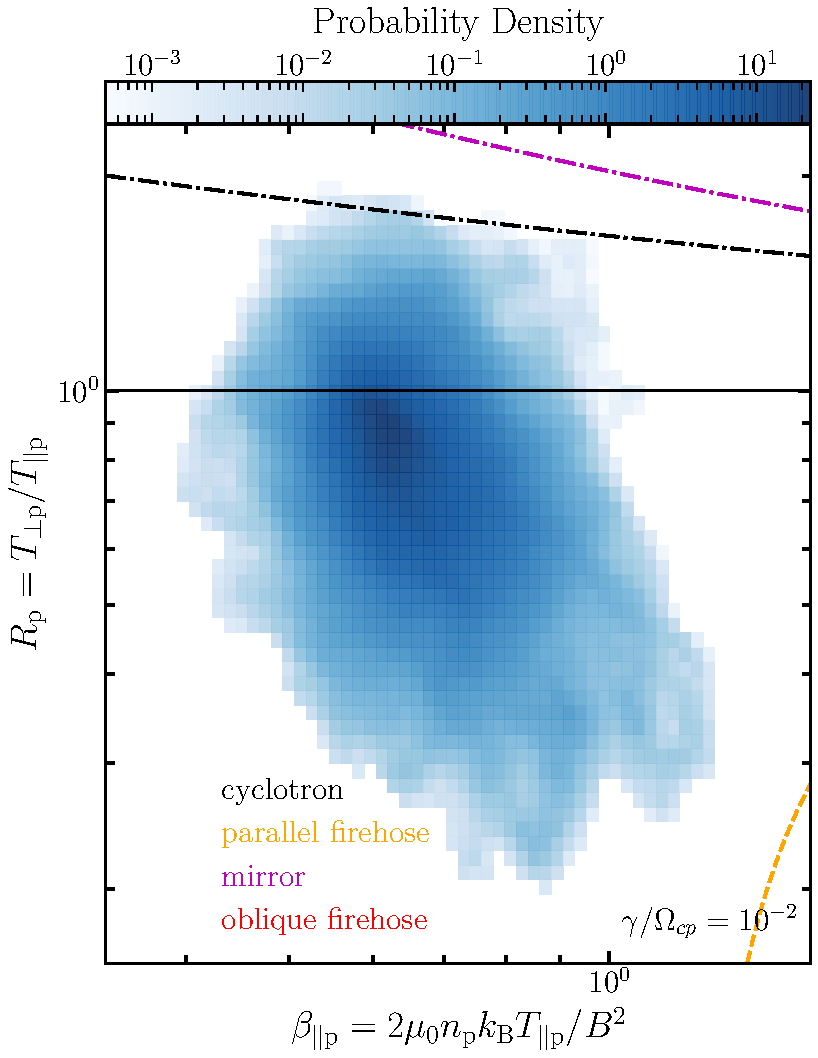
\includegraphics[width=1\textwidth]{figures/apdxA/brazil_prob_2dpp.pdf}
            \caption[Brazil-plot of \texttt{kaw} dataset]{Plot of estimated probability density,
            $\Tilde{p}$ of ($R_{\rm p}, \beta_{\parallel \rm p}$) for \texttt{kaw} dataset and
            thresholds associated with different instabilities for threshold value of
            $\gamma_{\max}/\Omega_{\rm cp} = 10^{-3}$.}
            \label{fig:brazil_prob_2dpp}
        \end{center}
    \end{figure}

    \begin{figure}
        \begin{center}
            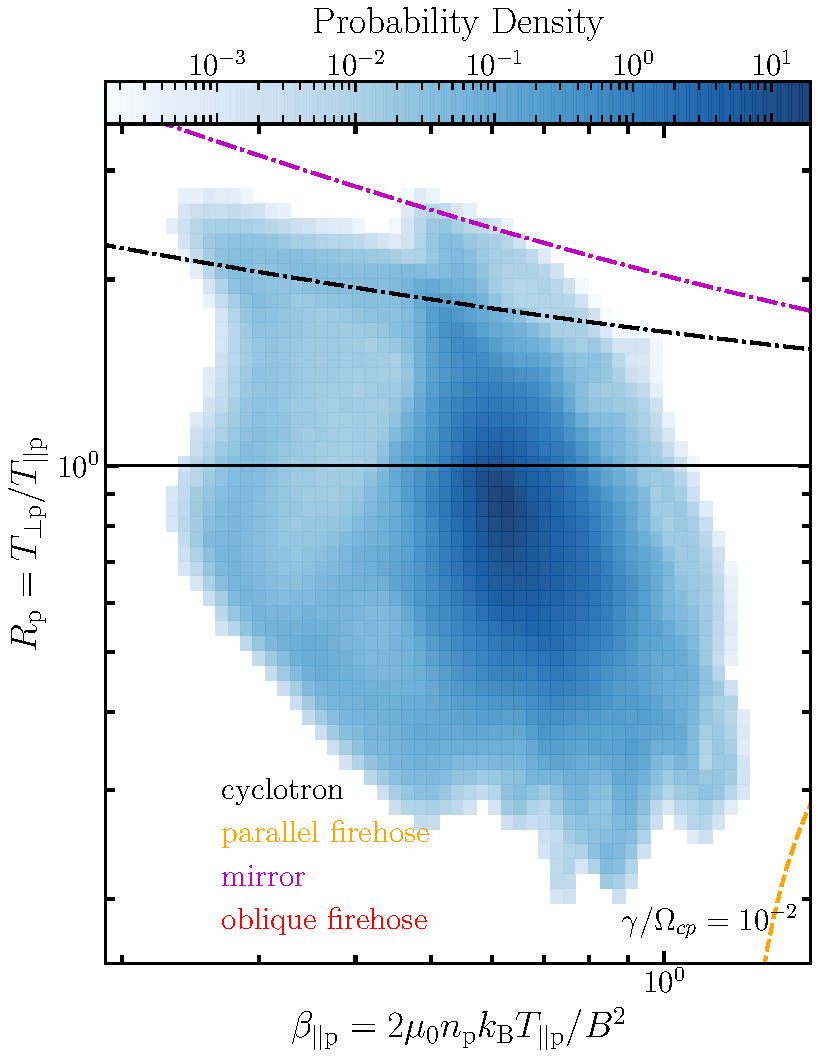
\includegraphics[width=1\textwidth]{figures/apdxA/brazil_prob_2d.pdf}
            \caption[Brazil-plot of \texttt{2dsim} dataset]{Plot of estimated probability density,
            $\Tilde{p}$ of ($R_{\rm p}, \beta_{\parallel \rm p}$) for combination of \texttt{149p6}
            and \texttt{kaw} dataset and thresholds associated with different instabilities for
            threshold value of $\gamma_{\max}/\Omega_{\rm cp} = 10^{-3}$.}
            \label{fig:brazil_prob_2d}
        \end{center}
    \end{figure}

    \begin{figure}
        \begin{center}
            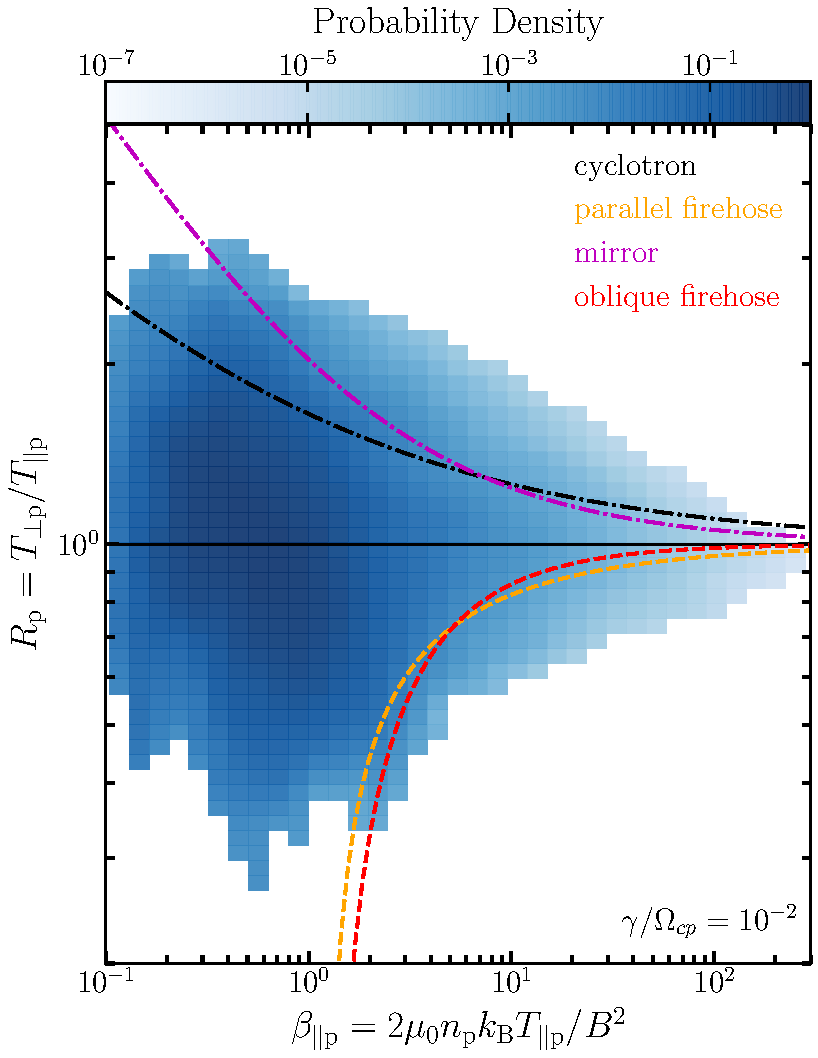
\includegraphics[width=1\textwidth]{figures/apdxA/brazil_prob_3d.pdf}
            \caption[Brazil-plot of \texttt{ros} dataset]{Plot of estimated probability density,
            $\Tilde{p}$ of ($R_{\rm p}, \beta_{\parallel \rm p}$) for \texttt{ros} dataset and
            thresholds associated with different instabilities for threshold value of
            $\gamma_{\max}/\Omega_{\rm cp} = 10^{-1}$.}
            \label{fig:brazil_prob_ros}
        \end{center}
    \end{figure}

    \begin{figure}
        \begin{center}
            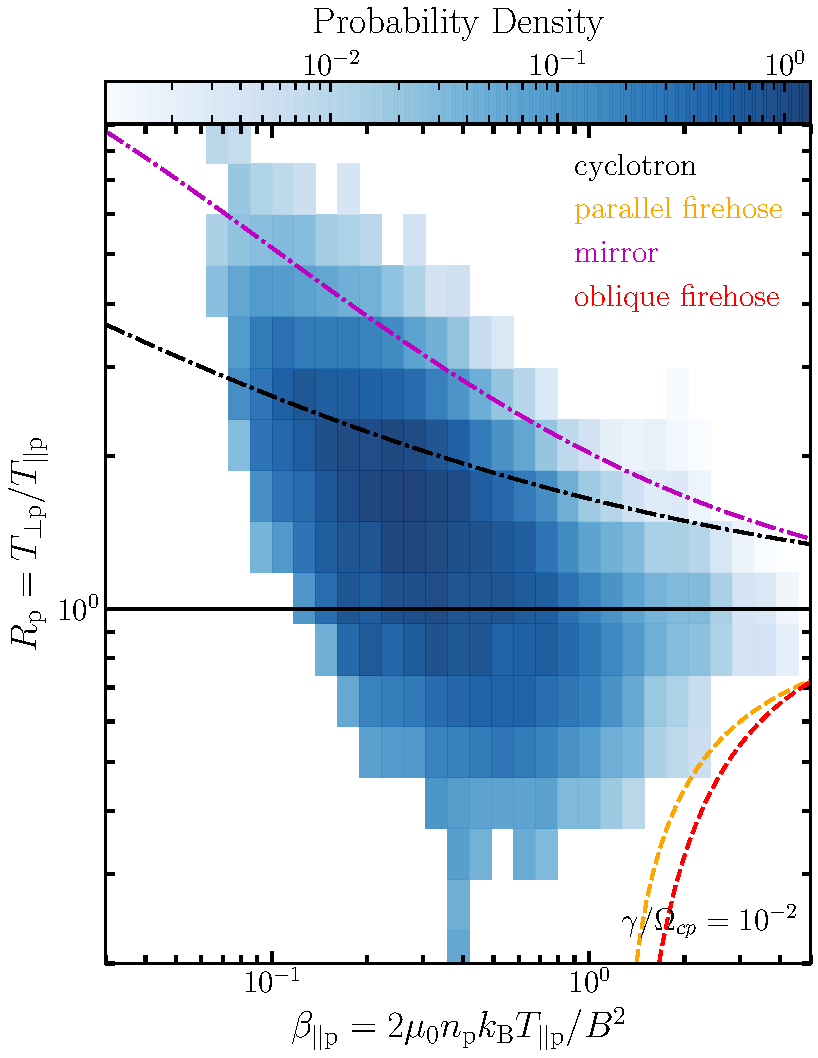
\includegraphics[width=1\textwidth]{figures/apdxA/brazil_prob_psp.pdf}
            \caption[Brazil-plot of \texttt{psp} dataset]{Plot of estimated probability density,
            $\Tilde{p}$ of ($R_{\rm p}, \beta_{\parallel \rm p}$) for \texttt{psp} dataset and
            thresholds associated with different instabilities for threshold value of
            $\gamma_{\max}/\Omega_{\rm cp} = 10^{-1}$.}
            \label{fig:brazil_prob_psp}
        \end{center}
    \end{figure}